\section{Ray-Tracing Dataset}
\label{sec:dataset}

The wireless channel dataset was generated using MATLAB's Ray Tracing
toolbox to provide independent validation of the results.


\subsection{MATLAB Ray-Tracing}
\label{sec:matlab_dataset}

The raw data for this exercise is from a ray tracing simulation done with a model of
central location in Otaniemi. The model was downloaded from Open Street Maps and all
the building walls were set to be concrete, roofs metal and ground as (MATLAB) loam in
Blender software. The antenna was left as ideal isotropic so we can add any antenna in
the post processing. The simulated area is $132 \times 147$ meters and the simulation was
done between 3\,069 receive and 9 transmit locations. The simulation was done with uniform
$2.5\,\text{m}$ grid which gives each location 8 equidistance neighbors. This needs to be
considered when later evaluating the performance of identifying neighbors. Maximum number
of reflections was set to four and the maximum number diffractions to two with the center
frequency of $3.6\,\text{GHz}$. This typically generated hundreds of paths per link in this
environment. 



\begin{figure}[htbp]
  \centering
  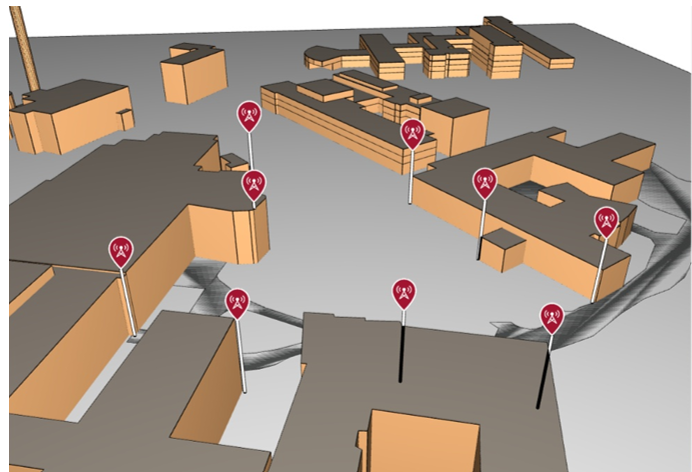
\includegraphics[width=0.8\columnwidth]{pictures/tommi/Simulated_environment.png}
  \caption{Simulated Otaniemi environment (132$\times$147\,m) showing
           the geographic area, building footprints, base station
           locations, and UE measurement grid.}
  \label{fig:tommi_environment}
\end{figure}

The $3\,069 \times 9$ simulation outputs were saved into individual JSON files that were
then consolidated into one $3\,069 \times 9 \times 5 \times 40$ matrix containing selected
information of 40 strongest paths from the raw data. The five kept vectors are: path real
part, imaginary part, azimuth angle of departure, elevation angle of departure and path
delay. The departure angle was used since we are later modelling signals coming from the
user equipment. This RT matrix was then saved into a file that could be used with our
feature creation algorithms. The feature creating algorithms can truncate the 40 path long
vectors to a more suitable length $N$, parameter used in the equations below. 

Ray tracing outputs themselves cannot be used as features since the real base station
would not have access to the signal in this format and fidelity. This raw data must be
then converted into real world receiver data. The base station has access to two useful
data vectors: (OFDM) CSI and (carrier) amplitude and phase of each antenna, ASI. We convert
the RT matrix into these two real world data vectors for the feature creation.

We calculated Antenna State Information for antenna $n,m$ as
\begin{equation}
  \text{ASI}[n,m] = \sum_{i=0}^{N} a_i e^{j\lambda(m \sin\theta_i \sin\varphi_i + n \sin\theta_i \cos\varphi_i)},
\end{equation}
where $\lambda$ is the antenna spacing in radians and $a$, $\varphi$, and $\theta$ are path
complex amplitude, azimuth and elevation angles from the RT matrix. We calculated the
response for various ULA and URA arrays for comparison. The antenna response itself can be
used as a feature in the form of flattened covariance matrix, or log-Euclidean distance
matrix between all receiver locations ($3\,096 \times 3\,096$). Our antenna program
generates both matrices.

While the antenna response covariance matrix can be used directly, the useful information
that it contains is in the angle of arrival. This means that the antenna data can be
compressed into more compact form that not only makes a smaller feature set, but also
suppresses a lot of noise and unnecessary information. While the original RT matrix contains
all this arrival angle information, it is not with a realistic resolution that the base
station antennas can see. Figure~\ref{fig:antenna_orientation} illustrates how coarse the
actual angle resolution is compared to the infinite resolution of the ray tracing.

We used Capon (Minimum Variance Distortionless Response) energy direction finding in 2D
and 1D to calculate more realistic arrival angles. Unless massive antenna arrays are used,
only the strongest direction contains useful information since the weaker paths are mostly
convoluted with the wide shoulders and sidebands of the main beam. The path phase contains
no coherent information, so it was also discarded. 

\begin{figure}[htbp]
  \centering
  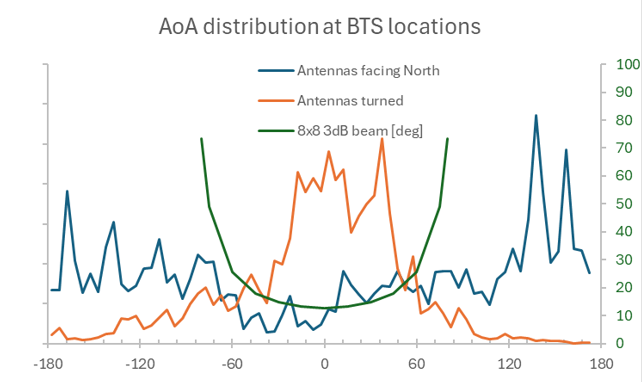
\includegraphics[width=\columnwidth]{pictures/tommi/Illustration_how_antenna_orientation_matters_when_wide_beams_are_used.png}
  \caption{Illustration how antenna orientation matters when wide beams are used. }
  \label{fig:antenna_orientation}
\end{figure}

As Figure~\ref{fig:antenna_orientation} shows, the beam resolution gets worse when turning
away from the antenna broadside, so the antennas were turned towards the center of the
area in interest.

The figure also shows how the azimuth angle distribution matches much better with the
accurate angle region after turning the antennas. We also allowed reception from the back
side of the antenna in the fingerprinting case. If the back side has strong radiation, then
those paths are aliased to the front side in the direction detection. In multi-angulation
the antenna was considered to have $180^\circ$ sector, so no back radiation was allowed.

MATLAB Phased Array library has \texttt{MVDREstimator2D()} function, but it turned out to
be performing poorly with the data from the ray tracing. So, the arrival angle estimation
was done in Python.

We calculated the CSI as
\begin{equation}
  \text{CSI}[n] = \sum_{i=0}^{N} a_i e^{j(n 2\pi f_s \tau_i + \varphi_i)},
\end{equation}
where $f_s$ is $15\,\text{kHz}$ and $n$ goes from $0$ to $6323$. Amplitude $a_i$ and phase
$\varphi_i$ are from the RT matrix. $\tau$ is also from the RT matrix but the true distance
is first subtracted from it and then a random number in $[0, 10\,\text{ns}]$ is added to mimic
a real receiver sampling. This will also prevent the (unknown) true distance from entering
the learning. All the LTE and 5G variants can be subsampled from this CSI vector. Again,
the CSI can be used as a feature on its own. If the CSI is used, then it can be further
downsampled since the coherence bandwidth is way larger than the subcarrier spacing. Also,
absolute value is as good as the full complex. The useful information that CSI contains is
in the path delays, amplitudes and (relative) phases. We used Matrix Pencil algorithm to
compress and extract the path information from the CSI. Delay statistics like mean delay
spread and spread variance can be then calculated from the extracted path information. Also,
the strongest three paths are saved as feature candidates. Strongest path time rank was
calculated after removing paths that are $10\,\text{dB}$ or more below the strongest.

All the possible options to create features from the simulation are illustrated in
Figure~\ref{fig:tommi_workflow}. Both the antenna and the frequency domain branches add
noise to the signal too. This is especially important in the frequency domain branch where
the path extraction would otherwise return the ideal ray tracing results due to the large
number of subcarriers. In the antenna branch the low number of antennas is more limiting
factor. Still, some diagonal loading needs to be done in Capon algorithm to avoid singular
matrices in good SNR samples. Also, some spatial smoothing was needed since the paths
correlate due to being from a single signal source. 

\begin{figure}[htbp]
  \centering
  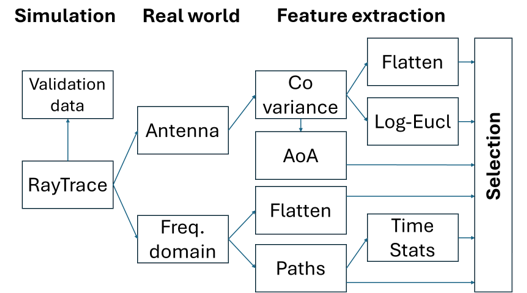
\includegraphics[width=\columnwidth]{pictures/tommi/Workflow_for_creating_the_features.png}
  \caption{Workflow for creating the features. Compressed data in grey. }
  \label{fig:tommi_workflow}
\end{figure}


\subsection{Data Compression and Features}

A key learning from this exercise was that some of the uncompressed data matrices, like
covariance and CSI, became too large to even read into computer memory. This gets easily
unmanageable when antenna count, base station count, sample count (resolution or area), or
channel bandwidth grows. Data compression becomes then the key, but the price is the
processing time that can be hours even for a small physical area. The right choice of
algorithm becomes critical and resolution versus processing time is the main tradeoff.

The following features and their dimensions are available for selection:

\begin{itemize}
  \item \textbf{Antenna\_aoa}: UE count $\times$ BTS count $\times$ [azimuth, elevation, amplitude]
  \item \textbf{Antenna\_cov}: UE count $\times$ [(antenna count$_{n}$ $\times$ antenna count$_{m}$ $\times$ BTS count)$^{2}$]
  \item \textbf{Antenna\_log\_euc}: UE count $\times$ UE count
  \item \textbf{Channel\_stats}: UE count $\times$ BTS count $\times$ [mean delay spread, delay spread variance, strong index, RSS, delay$[0]$, amplitude$[0]$, delay$[1]$, amplitude$[1]$, delay$[2]$, amplitude$[2]$]
  \item \textbf{CSI}: UE count $\times$ BTS count $\times$ [real $\times$ 798, imaginary $\times$ 798] at $50\,\text{MHz}/60\,\text{kHz}$
  \item \textbf{Validation}: UE count $\times$ [x, y, BTS count, LOS present]
  \item \textbf{Input\_data\_from\_Ray\_Trace}: UE count $\times$ BTS count $\times$ [real $\times$ 40, imaginary $\times$ 40, azimuth $\times$ 40, elevation $\times$ 40, delay $\times$ 40]; \texttt{zeros(5,40)} if no base station seen
\end{itemize}

\subsection{Sionna RT Dataset}
The Sionna\,RT dataset provides a physically calibrated characterisation
of the wireless channel with 27 multipath components per link and an RMS
delay spread of 191\,ns, consistent with measured sub-6\,GHz urban
propagation statistics~\cite{rappaport2013millimeter,3gpp_nr_channel}.
Detailed analysis of the multipath structure, including path-level
statistics, angular spread, and comparison with the independent MATLAB
ray-tracing validation dataset, is presented in the accompanying analysis
report (see Appendix~\ref{app:analysis_report}).
The validated dataset serves as the primary input to the fingerprint
localizer and the channel-charting pipeline in that document.